\documentclass[11pt,a4paper]{scrreprt}

\usepackage[utf8]{inputenc}
\usepackage[italian]{babel}

\usepackage{amsmath, amsfonts}
\usepackage{graphicx}

\usepackage{parskip}
\usepackage{color}

\usepackage{placeins}

\usepackage{url}

\newtheorem{teorema}{Teorema}
\newtheorem{lemma}[teorema]{Lemma}
\newtheorem{proposizione}[teorema]{Proposizione}
\newtheorem{proprieta}[teorema]{Proprietà}

\author{L. De Sano, A. Donizetti}
\title{\textsc{FIC}: Fractal Image Compression}
\date{Settembre 2015}

\begin{document}
\maketitle

\tableofcontents

\chapter{Introduzione}

Con il termine ``Fractal image Compression'' si va ad indicare una famiglia di tecniche di compressione di immagini (o video) basate sulle proprietà matematiche dei frattali. Tali metodi di compressione si rivelano sopra ogni altra cosa adatti a comprimere textures e immagini naturali, o, più in generale, immagini che sono caratterizzate da un elevato livello di \emph{self-similarity} (ovvero aventi delle parti che, al netto di rotazioni e ingrandimenti/riduzioni, somigliano ad altre parti dell'immagine).

La compressione di immagini tramite frattali (così come altre, più diffuse, ad esempio \textit{JPEG}) appartiene a quel gruppo di tecniche di compressione \emph{lossy}, ovvero in cui la compressione dell'immagine avviene al costo di una perdita di informazione. Tuttavia, a differenza di quanto accade quando si utilizza uno dei metodi di compressione basati sui pixel (come \textit{JPEG}, \textit{GIF} o \textit{MPEG}), nella compressione frattale nessuna parte dell'immagine viene effettivamente memorizzata. Ciò che viene memorizzato è invece la \emph{struttura interna} dell'immagine (ad esempio un indice di quali parti, effettuate le dovute trasformazioni, sono simili ad altre parti). 

Poiché nessun pixel dell'immagine originale viene memorizzato, la decompressione parte da un singolo pixel, di colore qualsiasi, e procede alla ricostruzione dell'immagine originale applicando iterativamente una mappa ricavata dalla struttura interna dell'immagine originale.

In questo documento tratteremo delle tecniche di compressione di immagini basate su frattali, iniziando con una panoramica teorica del loro funzionamento, proseguendo con la discussione di alcuni aspetti pratici e presentando una implementazione giocattolo realizzata in MATLAB, e concludendo infine con alcuni test che consentiranno di valutare praticità e \emph{performances} di una libreria di compressione basata su frattali, anche in confronto con altre tecniche di compressione \emph{lossy} maggiormente utilizzate.

\chapter{Aspetti teorici}

\section{Introduzione ai frattali}

Un frattale è un oggetto geometrico che si ripete nella sua forma, allo stesso modo, su diverse scale. Questo comportamento fa si che ingrandendo una sua qualsiasi componente, ciò che si ottiene è una figura simile all'originale. In linea di massima, si può dire che perché l'insieme $F$ sia considerato un frattale, $F$ dovrebbe avere almeno le seguenti proprietà:

\begin{itemize}
\item $F$ ha dettagli ad ogni scala d'ingrandimento;
\item $F$ gode di autosimilitudine (a qualunque scala si osservi, presenta sempre le stesse caratteristiche globali);
\item la dimensione frattale di $F$ è maggiore della sua dimensione topologica;
\item esiste un algoritmo relativamente semplice per costruire $F$.
\end{itemize}

{\color{red} TODO: definire dimensione frattale e topologica}

\url{http://www.vanderbilt.edu/AnS/psychology/cogsci/chaos/workshop/Fractals.html}

% mettere qualche esempio di frattale di base con la costruzione iterata?

Un esempio di oggetto geometrico secondo i principi di costruzione di un frattale e che rispetta le proprietà elencate è la curva di \textit{Koch}. La costruzione comincia con una linea di lunghezza $1$ chiamata \textit{initiatior}. Da questa linea si rimuove il terzo centrale e lo si sostituisce con due linee della stessa lunghezza della parte rimossa. Questa nuova forma viene chiamata \textit{generator}. La prima parte della costruzione è mostrata in figura \ref{fig:k1}.

\begin{figure}[!ht]
\centering
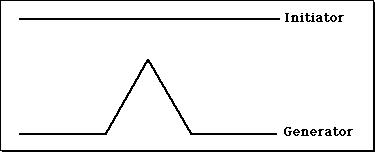
\includegraphics[scale=0.55]{images/koch1.png}
\caption{Initiator e generator per la curva di Koch}
\label{fig:k1}
\end{figure}

La regola può essere nuovamente applicata su ogni linea, così da andare a sostituirla ogni volta come fanno nel passaggio da \textit{initiator} a \textit{generator}. Il secondo livello è visibile in figura \ref{fig:k2}.

\begin{figure}[!ht]
\centering
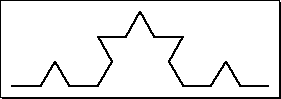
\includegraphics[scale=0.55]{images/koch2.png}
\caption{Livello 2 per la curva di Koch}
\label{fig:k2}
\end{figure}

\FloatBarrier

Una volta che la procedura è avviata può proseguire a piacimento. Il terzo e il quarto livello sono visibili nelle figure \ref{fig:k3} e \ref{fig:k4} rispettivamente.

\begin{figure}[!ht]
\centering
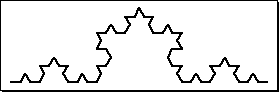
\includegraphics[scale=0.55]{images/koch3.png}
\caption{Livello 3 per la curva di Koch}
\label{fig:k3}
\end{figure}

\begin{figure}[!ht]
\centering
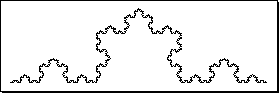
\includegraphics[scale=0.55]{images/koch4.png}
\caption{Livello 4 per la curva di Koch}
\label{fig:k4}
\end{figure}



\section{Iterated Function Systems}

Uno strumento matematico che si rivelerà fondamentale nella fase di decompressione delle immagini trattate con un metodo di compressione frattale è quello degli \emph{Iterated Function Systems}, che andiamo per questo motivo a descrivere qui.

Senza eccedere in formalità, definiamo un \emph{Iterated Function System} (IFS) come una collezione di trasformazioni contrattive $\{w_i : \mathbb{R}^2 \rightarrow \mathbb{R}^2 \}_{i=1,\ldots, n}$ che mappa il piano su se stesso. Questa collezione di trasformazioni definisce una mappa 

\[
W(\cdot) = \bigcup_{i=1}^{n} w_i(\cdot)
\]

Tale mappa è applicata ad insiemi di punti, ed il risultato è definito in questa maniera: dato un insieme di punti $S \in \mathbb{R}^2$, calcoliamo $w_i(S)$ per ogni $i$ (ovvero produciamo $i$ copie ridotte di $S$), e poi calcoliamo l'unione dei risultati (ovvero, mettiamo insieme tutte le copie ridotte), ottenendo così un nuovo insieme $S' = W(S)$.

$W$ così definito è una mappa tra sottoinsiemi di $\mathbb{R}^2$ (che d'ora in avanti per noi saranno ``immagini''), e gode di due importanti (e rilevanti per la compressione frattale) proprietà, che andiamo ad enunciare senza dimostrazione.

\begin{proprieta}
Se tutte le $w_i$ sono contrattive, allora $W$ è contrattiva in uno spazio di sottoinsiemi del piano.
\end{proprieta}

\begin{proprieta}
Fissata una mappa $W$, esiste una immagine $x_W$, chiamata \emph{attrattore per $W$}, tale che
\begin{itemize}
\item $W(x_W) = x_W$
\item data una qualunque immagine di partenza $S_0$, vale che 
\[x_W \equiv \lim_{n \rightarrow \infty} W^{n}(S_0) \]
ovvero l'applicazione ripetuta per $n$ volte di $W$ porta ad ottenere $x_W$, per $n$ sufficientemente grande, ed indipendentemente dalla scelta dell'immagine di partenza.
\item $x_W$ è unica. Se una qualsiasi immagine $S$ soddisfa $W(S) = S$, allora $S$ è l'attrattore per $W$.
\end{itemize}
\end{proprieta}

La seconda di queste proprietà è nota come \emph{Contractive Mapping Fixed-Point Theorem}.

\section{Self-similarity nelle immagini}

\subsection*{Immagini come oggetti matematici}

Per poter applicare la teoria degli \emph{IFS} alle immagini come comunemente le intendiamo (ovvero, in sostanza, matrici di pixels rappresentati  da 1 byte -- \emph{greyscale} -- oppure più di uno -- es. RBG --), è necessario formalizzare in qualche modo il concetto di ``immagine digitale'', cercando di inserirlo in un contesto matematico che ci consenta di manipolarla utilizzando di strumenti messi a disposizione dall'algebra. Per semplicità, ci limiteremo qui a considerare le immagini in \emph{grayscale} (un singolo canale di colore, l'intensità indicata con un numero da 0 a 255).

Consideriamo un'immagine in scala di grigi, memorizzata come matrice di pixel, 1 byte per ogni pixel. Non è difficile immaginare di poter rappresentare tale immagine utilizzando una funzione $f: \mathbb{R}^2 \rightarrow  \{1, 2, \ldots, 255 \}$, in modo tale che ad ogni pixel alle coordinate $(x, y)$ sia fatto corrispondere un punto $(x, y)$ nel piano, al quale a sua volta viene associata un'altezza $z$, che corrisponde al valore di grigio del pixel in questione. 

Ad esempio, ad un'immagine con il primo pixel in basso a sinistra avente livello di grigio 177, viene fatta corrispondere una funzione $f$ che, per quanto riguarda quel preciso punto, avrà $f(0,0) = 177$. Effettuando questa operazione su tutti i pixel dell'immagine originale, è possibile definire completamente $f$ su tutta la parte del piano di nostro interesse (e, in genere, si riduce per convenzione l'immagine ad avere dominio 
$[0, 1]^2$). Nella figura qui sotto riportata si può vedere un esempio del risultato finale della procedura, applicata ad una immagine grayscale $128 \times 128$ pixels.

\begin{figure}[!ht]
\centering
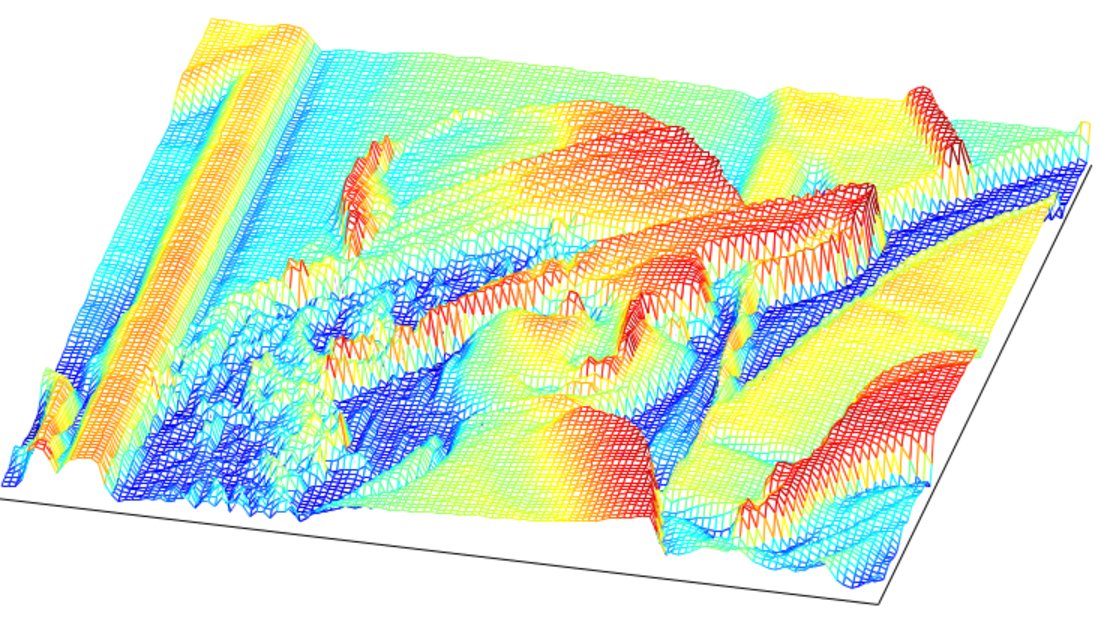
\includegraphics[scale=0.6]{images/lena-mash.pdf} 
\caption{lena grayscale, $128 \times 128$ pixels, trasformata in funzione $[0,1]^2 \rightarrow \{0,\ldots,255 \}$}
\end{figure}

La trasformazione descritta ci permette di ignorare l'aspetto ``visivo'' della modalità in cui una immagine è memorizzata, e ci consente di identificare una immagine con la funzione $f$ associata, su cui si andrà ad operare durante il procedimento di compressione.

\subsection*{Distanza tra due immagini}

Un secondo concetto che è necessario introdurre per poter operare sulle immagini durante il procedimento di compressione e decompressione è quello di ``distanza'' tra due immagini. La contrattività di una mappa $W$ (ovvero, intuitivamente, il fatto che essa rende le immagini più ``piccole'') può essere verificata solo se si ha a disposizione una qualche metrica sulla base della quale è possibile valutare la distanza tra due sottoinsiemi del piano (ovvero, nel nostro caso, due immagini).

Date due immagini $f, g$, definiamo la loro distanza $d(f, g)$, utilizzando la media quadratica, come

\[
d(f,s) = \sqrt{\int_{[0,1]^2} f(x,y) - g(x,y) \quad \text{d}x\text{d}y }
\]

La metrica ci fornisce una maniera di valutare la distanza tra due immagini pesando in maniera uniforme tutti i punti in esse contenuti.

\subsection*{Self-similarity debole}

A differenza di quanto accade quando si osserva un frattale vero e proprio, all'interno di immagini ``naturali'' non troviamo una \emph{self-similarity} forte: solitamente non abbiamo parti dell'immagine che sono simili all'immagine complessiva, bensì parti dell'immagine che sono simili ad altre parti dell'immagine. Un altro aspetto da considerare è quello della colorazione: due parti dell'immagine potrebbero essere simili nella composizione dei pixel, ma differenti per quanto riguarda la gradazione di grigio dei pixels che le compongono. 

I basilari IFS che abbiamo descritto in precedenza vanno leggermente complicati, nel contesto della compressione frattale delle immagini, in modo da accomodare i due aspetti qui sopra descritti. Come prima cosa, notiamo che al momento di definire le trasformazioni $w_i$, dovremo fare in modo che ad ogni trasformazione sia consentito di andare a toccare solo un particolare sottoinsieme del piano, in maniera da accomodare il requisito di poter rappresentare la \emph{self-similarity} debole (similarità tra parti e altre parti, e non con l'intera immagine). Come seconda cosa, alle mappe vanno aggiunti due parametri, \emph{contrasto} e \emph{luminosità}, che ci consentiranno di definire non solo trasformazioni  \emph{spaziali}, ma anche trasformazioni che vanno a coinvolgere la differenza di \emph{colorazione} (sempre su scala di grigi) tra due sottoinsiemi di piano.

Invece della classica trasformazione su $\mathbb{R}^2$ che ci aspetteremmo considerato il fatto che stiamo operando su funzioni $\mathbb{R}^2 \rightarrow \mathbb{R}$, definiamo le $w_i$ come trasformazioni su $\mathbb{R}^3$:

\[
w_i \begin{bmatrix} 
x \\
y \\
z
\end{bmatrix} = \begin{bmatrix}
a_i & b_i & 0 \\
c_i & d_i & 0 \\
0 & 0 & s_i \\
\end{bmatrix} \cdot \begin{bmatrix} 
x \\
y \\
z
\end{bmatrix} + \begin{bmatrix} 
e_i \\
f_i \\
o_i
\end{bmatrix}
\]

La trasformazione è formata da una componente \emph{spaziale}, ovvero

\[
v_i \begin{bmatrix} 
x \\
y \\
\end{bmatrix} = \begin{bmatrix}
a_i & b_i \\
c_i & d_i \\
\end{bmatrix} \cdot \begin{bmatrix} 
x \\
y \\
\end{bmatrix} + \begin{bmatrix} 
e_i \\
f_i \\
\end{bmatrix}
\]

e di due parametri aggiuntivi $s_i$ ed $o_i$, che agiscono rispettivamente come moltiplicatore e scala tramite somma sulla componente $z$ della funzione. Questi due parametri, che chiamiamo rispettivamente \emph{contrasto} e \emph{luminosità}, non influenzano in alcun modo le componenti spaziali della trasformazione, e ci consentono di definire trasformazioni sullo spazio di \emph{colore} dell'immagine (che, ricordiamo, è rappresentato nella funzione associata all'immagine come la componente $z$). 

Ricordando che l'immagine è rappresentata da una funzione $z = f(x,y)$, dove $x$ ed $y$ sono pixels e $z$ il grado di grigio dell'immagine \emph{grayscale}, una singola trasformazione $w_i$ viene applicata calcolando $w_i(f) = w_i(x, y, f(x,y))$. La parte spaziale di $w_i$ determina come una sotto-parte dell'immagine è mappata su altre sottoparti, mentre $s_i$ ed $o_i$ determinano contrasto e luminosità della trasformazione.

Il fatto che il mapping sia da effettuarsi da sottoinsiemi a sottoinsiemi dell'immagine è permesso dal fatto che le varie $w_i$ sono implicitamente definite in modo da operare su un sottoinsieme di $[0,1]^2$, che chiamiamo $D_i$, dando come risultato un sottoinsieme di $[0,1]^2$, che chiameremo $R_i$. In simboli, scriviamo che

\[
v_i(D_i) = R_i
\]

ovvero la componente spaziale della trasformazione ha dominio in sottoinsiemi del piano che chiamiamo $D_i$ e codominio in sottoinsiemi del piano che chiamiamo $R_i$.

Poiché richiediamo che $W(f)$, l'unione delle $w_i$, sia a sua volta un'immagine compatta, le trasformazioni devono soddisfare due proprietà basilari: prima di tutto gli $R_i$ devono partizionare completamente $[0,1]^2$, ovvero deve valere $\bigcup_i R_i = [0,1]^2$. Inoltre gli $R_i$ non devono sovrapporsi, ovvero deve valere $R_i \not= R_j$ se $i \not= j$. Queste due proprietà garantiscono che l'applicazione della mappa $W$ su una immagine $S$ risulti in una immagine $S'$, possibilmente differente, ma completa ed univoca.

Poiché la mappa $W$ è contrattiva solo se lo sono le trasformazioni $w_i$, è necessario scegliere accuratamente i parametri di queste ultime. Dato che la metrica di distanza $d$ che abbiamo definito sopra non prende in considerazione le direzioni $x$ ed $y$, ma soltanto la direzione $z$, per assicurare la contrattività delle $w_i$ è sufficiente fare attenzione al parametro di scala $s_i$. In particolare:

\begin{proprieta}
Le trasformazioni $w_i$ sono contrattive per $s_i < 1$
\end{proprieta}

\subsection*{Decoding}

A questo punto abbiamo tutti gli strumenti che servono per effettuare il \emph{decoding} di una immagine compressa utilizzando frattali: partendo  da una immagine qualunque, si applica ripetutamente la mappa $W$ fino a quando non si raggiunge il suo punto fisso $x_W$, che rappresenta il risultato dell'operazione di decodifica.

L'aspetto interessante (e complicato) della tecnica di compressione che stiamo descrivendo è però un altro: come fare, data una immagine $f$ da comprimere, a trovare un insieme di mappe $\{w_i\}_i$ tale che $f$ sia il punto fisso della loro unione ($W$)? Questa operazione, che rappresenta il nucleo delle tecniche di compressione tramite frattali, è l'argomento della prossima sezione.

\section{Encoding}

Come anticipato nella precedente sezione, per comprimere un'immagine $f$ è necessario trovare una mappa $W$ tale che 

\[
f = W(f)
\]

ovvero una mappa $W$ avente $f$ come attrattore. Ricordando la definizione di $W$, la proprietà richiesta diventa

\[
f = w_1(f) \cup w_2(f) \cup \dots \cup w_N(f)
\]

Per ottenere questo, dovremmo procedere con il partizionare l'immagine $f$ in tanti pezzi tali per cui, applicando le trasformazioni $\{w_i\}_i$, si otterrebbe l'immagine di partenza. Chiaramente, in generale, questa è una condizione troppo restrittiva: ottenere \emph{esattamente} l'immagine di partenza non è qualcosa che sia possibile sperare (a parte nei casi in cui si stia cercando di comprimere un'immagine frattale!).

Quello che facciamo in pratica è cercare delle trasformazioni che, applicate, ci restituiscano un'immagine \emph{differente}, diciamo $f'$, tale per cui la distanza con l'immagine di partenza, ovvero $d(f,f')$, è piccola. Operativamente, procediamo calcolando le $w_i$ con l'obbiettivo di minimizzare la distanza tra il pezzo di immagine che stiamo attualmente considerando e il pezzo di immagine ottenuto dopo l'applicazione della trasformazione. In formula, minimizziamo

\[
d\big(f \cap (R_i \times I), w_i(f)\big) 
\]

per tutti gli $i$.

\subsection*{Partizionare le immagini}

\chapter{Aspetti Pratici e di implementazione}


\chapter{Test, benchmarks}


\end{document}
